%%% Uppsala University presentation beamer template v2.0
%%% provided by Diletta Goglia, IT Department, Uppsala University
%%% email: diletta.goglia@it.uu.se
%%% December, 2023

% This template is the updated version of the "Uppsala University presentation template v1.0" created by Mats Jonsson (mats@mekeriet.se) in March 2021.


\documentclass{beamer}


\usepackage[english]{babel}
\usepackage[utf8x]{inputenc}
\usepackage{hyperref, % clickable links
    graphicx, % include images
    listings, % for code and formatting
    caption, % customization of captions in figures and tables
    stackengine, % custom layouts 
    amsmath, % math env
    xcolor, % extend color support
    multicol, % multiple columns layout
    booktabs, % high quality tables
    lipsum % remove it
}

%\usepackage{UU_beamer} % customized style




%\usetheme{default}
%\usetheme{AnnArbor}
%\usetheme{Antibes}
%\usetheme{Bergen}
%\usetheme{Berkeley}
%\usetheme{Berlin}
%\usetheme{Boadilla}
%%%%%%%%%\usetheme{CambridgeUS}
%\usetheme{Copenhagen}
%\usetheme{Darmstadt}
%\usetheme{Dresden}
%\usetheme{Frankfurt}
%\usetheme{Goettingen}
%\usetheme{Hannover}
%\usetheme{Ilmenau}
%\usetheme{JuanLesPins}
%\usetheme{Luebeck}
%%%%%\usetheme{Madrid}
%\usetheme{Malmoe}
%%%%%%%%%%%%%%%%%\usetheme{Marburg}
%\usetheme{Montpellier}
%\usetheme{PaloAlto}
%%%%%\usetheme{Pittsburgh}
%\usetheme{Rochester}
\usetheme{Singapore}
%\usetheme{Szeged}
%\usetheme{Warsaw}
%\usetheme{boxes}




\def\cmd#1{\texttt{\color{red}\footnotesize $\backslash$#1}}
\def\env#1{\texttt{\color{blue}\footnotesize #1}}

% ------ CODE COLOR DEFINITION ------ %

\definecolor{codered}{rgb}{0.6,0,0}
\definecolor{codeblue}{rgb}{0,0,0.8}
\definecolor{codegreen}{rgb}{0,0.5,0}
\definecolor{almostwhite}{gray}{0.55}
\definecolor{codepurple}{rgb}{0.58,0,0.82}
\definecolor{backcolour}{rgb}{0.95,0.95,0.92}

\lstset{
    basicstyle=\ttfamily\small,
    keywordstyle=\bfseries\color{codeblue},
    emphstyle=\ttfamily\color{codered},   % Custom highlighting style
    stringstyle=\color{codepurple},
    numbers=left,
    numberstyle=\small\color{almostwhite},
    rulesepcolor=\color{red!20!green!20!blue!20},
    frame=shadowbox,
    commentstyle=\color{codegreen},
    captionpos=b    
}

% ------------- PRESENTATION INFO --------------- %
\newcommand{\fullconference}{Memory Technologies - Spring 2024}
\newcommand{\shortconference}{MT - Spring 2024}
\newcommand{\contact}{\textit{\href{mailto:adinepour@aut.ac.ir}{adinepour@aut.ac.ir}}}

\author[RA, \contact]{\href{}{Reza Adinepour}}
\institute[CE Department, AUT]{\href{}{Computer Engineering Department, Tehran Ploytechnic}
    \\ \smallskip \contact}
\title[Exploring Memory Technology Simulators]{Exploring Memory Technology Simulators}
\subtitle[\shortconference]{}
\date[Month 20XX]{\small \today
    \\ \fullconference}


\begin{document}

% ------------ TITLE SLIDE --------------- %
{
% Remove headline and footline from first slide
\setbeamertemplate{footline}{} 
\setbeamertemplate{headline}{} 

\begin{frame}\label{start}
    \titlepage
    \begin{figure}
            
\includegraphics[scale=0.13]{style/uu_logo} 
    \end{figure}
\end{frame}
}

% ---------- TABLE OF CONTENT --------- %
\begin{frame}{Agenda}
    \tableofcontents[sectionstyle=show, subsectionstyle=show/shaded/hide, subsubsectionstyle=show/shaded/hide]
\end{frame}




% --------- SECTION 4 ------- %
\section{DRAMSIM}

\begin{frame}{DRAMSIM}
	\begin{enumerate}
		\item DRAMSim use for simulate Dynamic RAMs.
		\begin{enumerate}
			\item DRAM modeling it's very important because the technology is trying to provide CPU and DRAM integrated in one chip.
			\item This provides high density:
			\begin{enumerate}
				\item High density
				\item Optimal performance
				\item Lower power consumption
			\end{enumerate}
		\end{enumerate}
		\item DRAMSim is provide in three version:
		\begin{enumerate}
			\item DRAMSim 1
			\item DRAMSim 2
			\item DRANSim 3\\
			\textbf{In this talk, we discuss about the last version of DRAMSim}
		\end{enumerate}
		\item DRAMSim developed in C++ and write in modularly.
	\end{enumerate}
\end{frame}





\begin{frame}{DRAMSIM (Cont.)}
	\begin{enumerate}
		\item DRAMSim can be connected to GEM5
		\item DRAMSim can simulate following protocol:
		\begin{enumerate}
			\item DDR3
			\item DDR4
			\item ‫‪LPDDR3‬‬
			\item ‫‪LPDDR4‬‬
			\item ‫‪GDDR5‬‬
			\item ‫‪GDDR6‬‬
			\item HBM
			\item HMC
			\item ‫‪STT-MRAM‬‬
		\end{enumerate}
	\end{enumerate}
	
	The structure of main block of DRAMSim is shown in figure \ref{fig:Main block of DRAMSim}.
\end{frame}



\begin{frame}{DRAMSIM (Cont.)}
	\begin{figure}
		\centering
		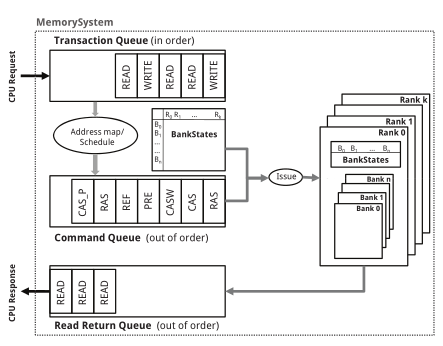
\includegraphics[height=6cm]{images/img11}
		\caption{Main block of DRAMSim}
		\label{fig:Main block of DRAMSim}
	\end{figure}
\end{frame}




\begin{frame}{DRAMSIM (Cont.)}
	\textcolor{green}{Advantages:}
	\begin{enumerate}
		\item The possibility of simulating new DRAM technologies like DDR4 and GDDR6
		\item High flexibility in configuration
		\item Synchronize with system simulators
	\end{enumerate}
	
	\textcolor{red}{Disadvantages:}
	\begin{enumerate}
		\item Dependence on the model and configuration
		\item Don't report power consumption and area
	\end{enumerate}
\end{frame}







\begin{frame}{DRAMSIM (Cont.)}
	\textbf{How install and build DRAMSim?}\\
	We should clone repository in first step:
	\begin{block}{Clone repository}
		\texttt{\textcolor{blue}{\$} git clone ‫‪https://github.com/umd-memsys/DRAMsim3‬‬} \\
		\texttt{\textcolor{blue}{\$} ‫‪DRAMsim3‬‬‫‪cd‬‬} \\
	\end{block}
	
	now we should build it:
	\begin{block}{Build}
		\texttt{\textcolor{blue}{\$} mkdir build‬‬} \\
		\texttt{\textcolor{blue}{\$} ‫‪cd build‬‬‫‪cd‬‬} \\
		\texttt{\textcolor{blue}{\$} ‫‪cmake ..‬‬} \\
		\texttt{\textcolor{blue}{\$} ‫‪make -j4‬‬} \\
		\texttt{\textcolor{blue}{\$} ‫‪‫‪-DTHERMAL=1‬‬‫‪..‬‬ ‫‪cmake‬‬‬‬} \\
	\end{block}
\end{frame}




\begin{frame}{DRAMSIM (Cont.)}
	If the simulation builds successfully, you can see \textbf{Built target} on your terminal like figure \ref{fig:DRAMSim built target}
	
	\begin{figure}
		\centering
		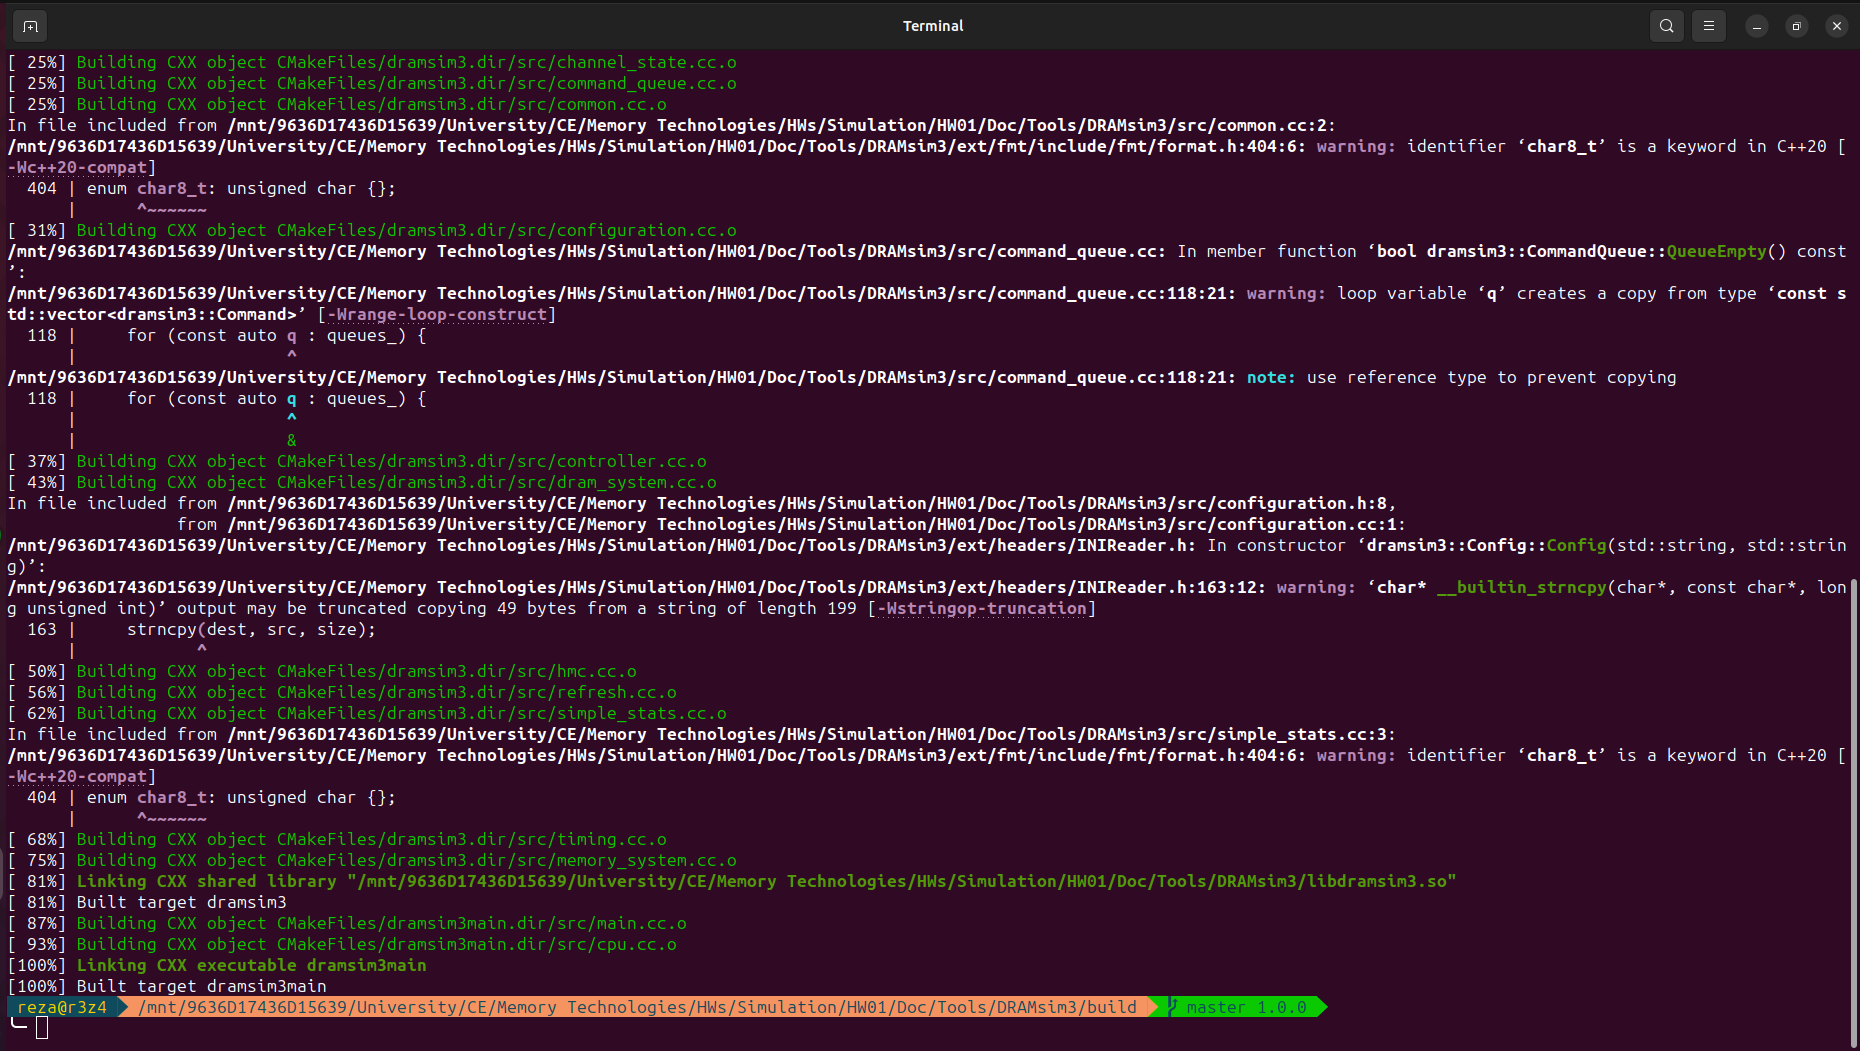
\includegraphics[height=5cm]{images/img12}
		\caption{DRAMSim built target}
		\label{fig:DRAMSim built target}
	\end{figure}
\end{frame}


\begin{frame}{DRAMSIM (Cont.)}
	\textbf{How can run sample simulation?}\\
	\begin{enumerate}
		\item in first, create a folder for save output file of simulation:
		\begin{block}{Create output directory}
			\texttt{\textcolor{blue}{\$} ‫‪‬‬‫‪mkdir output‬‬‬‬} \\
		\end{block}
		
		\item then, with this command, run simulation for \texttt{sample\_trace.txt} config file:
		\begin{block}{Run simulation}
			\texttt{\textcolor{blue}{\$} ‫‪./build/dramsim3main‬‬ ‫‪configs/DDR4\_8Gb\_x8\_3200.ini -c‬‬‬‬‬‬ 100000 -t tests/‫‪example\_trace.txt‬‬ -o output/} \\
		\end{block}		
	\end{enumerate}
	every various configurations files, located in \texttt{configs/} directory. for this simulation we use \texttt{DDR4\_8Gb} config file.
\end{frame}


\begin{frame}{DRAMSIM (Cont.)}
	after simulation is finished, you can see output in \texttt{output/} directory in \texttt{dramsim3.txt} file like bellow:
	\begin{figure}
		\centering
		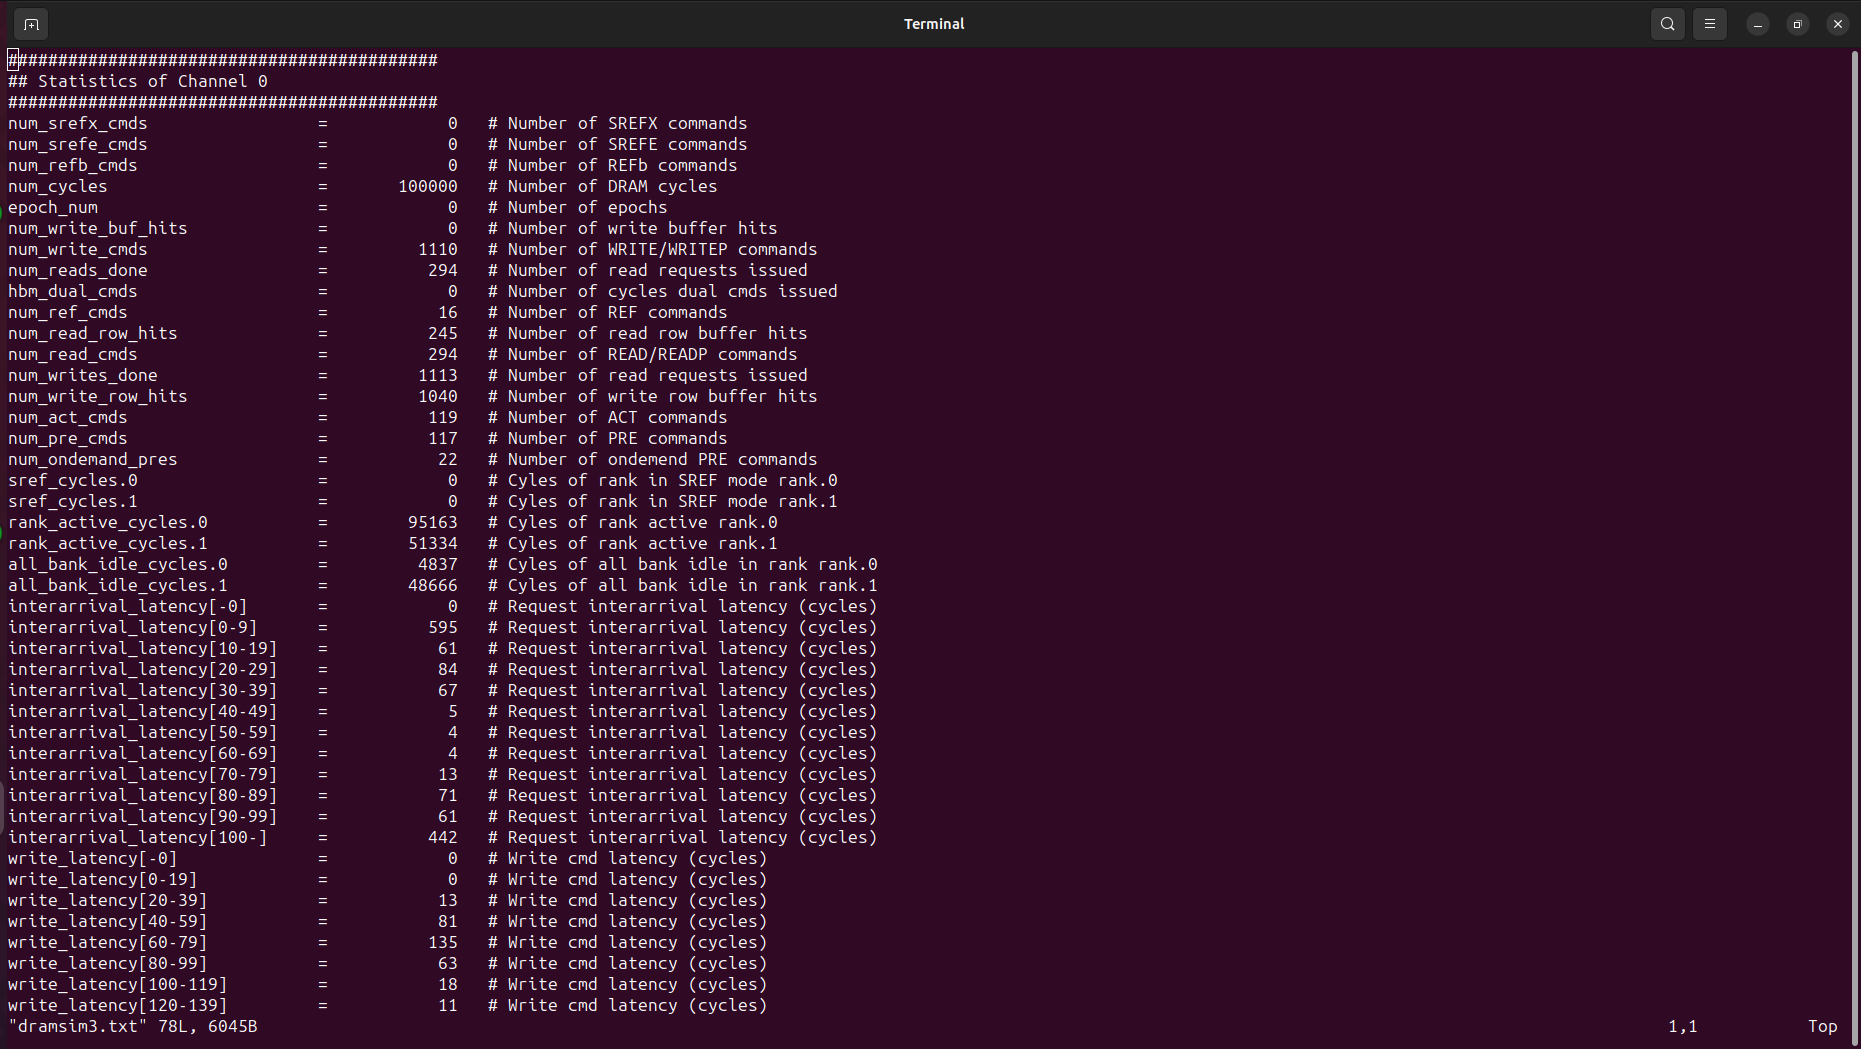
\includegraphics[height=5cm]{images/img12_2}
		\caption{Output report}
		\label{fig:Output report of DRAMSim}
	\end{figure}
\end{frame}



\begin{frame}{DRAMSIM (Cont.)}
	we can plot read latancy, interarrival latancy, write latancy and ... with some python scripts located in \texttt{script/} directory.
	
	\begin{block}{plot}
		\texttt{\textcolor{blue}{\$} python3 scripts/plot\_stats.py output/dramsim3.json‬‬} \\
	\end{block}
	
	the output of simulation:	
\end{frame}




\begin{frame}{DRAMSIM (Cont.)}
	\begin{figure}
		\centering
		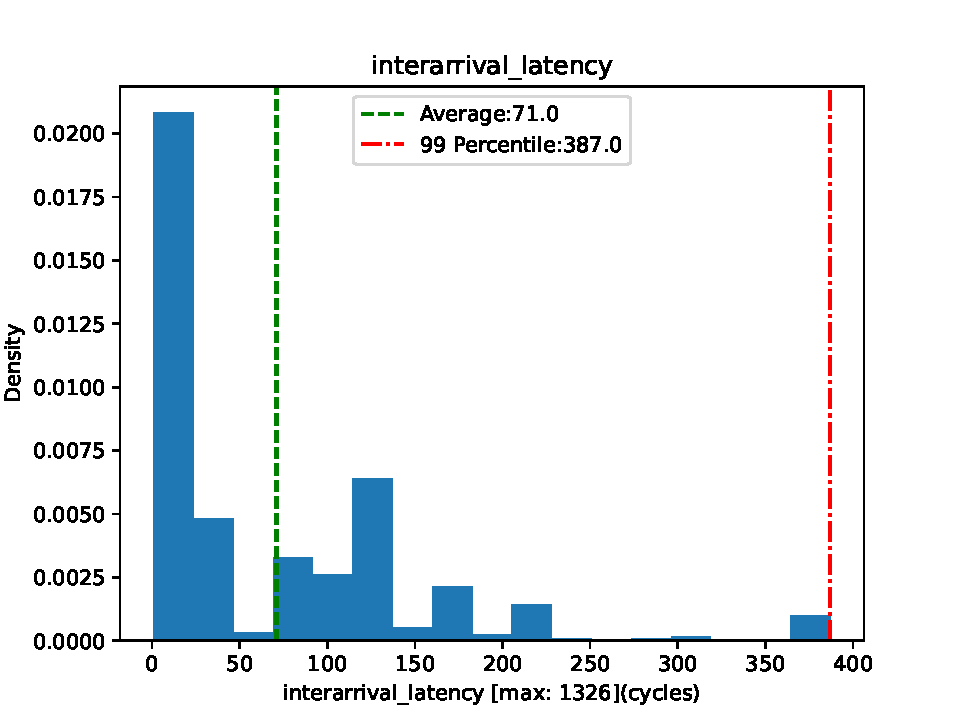
\includegraphics[height=6cm]{images/img13}
		\caption{Interarrival latancy}
		\label{fig:Interarrival latancy}
	\end{figure}	
\end{frame}



\begin{frame}{DRAMSIM (Cont.)}
	\begin{figure}
		\centering
		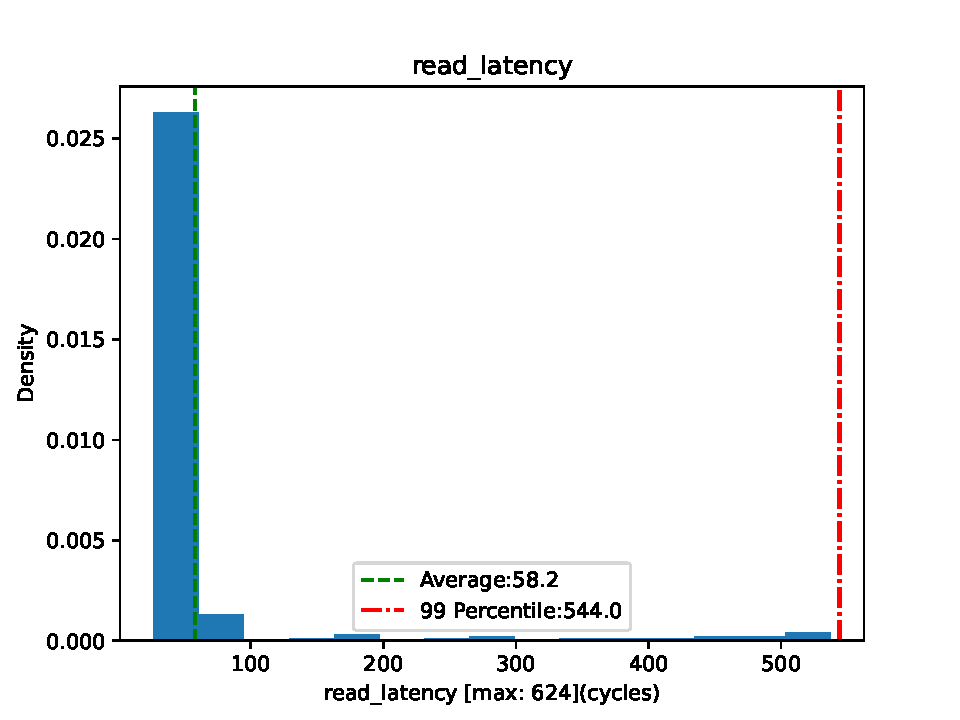
\includegraphics[height=6cm]{images/img14}
		\caption{Read latancy}
		\label{fig:Read latancy}
	\end{figure}	
\end{frame}


\begin{frame}{DRAMSIM (Cont.)}
	\begin{figure}
		\centering
		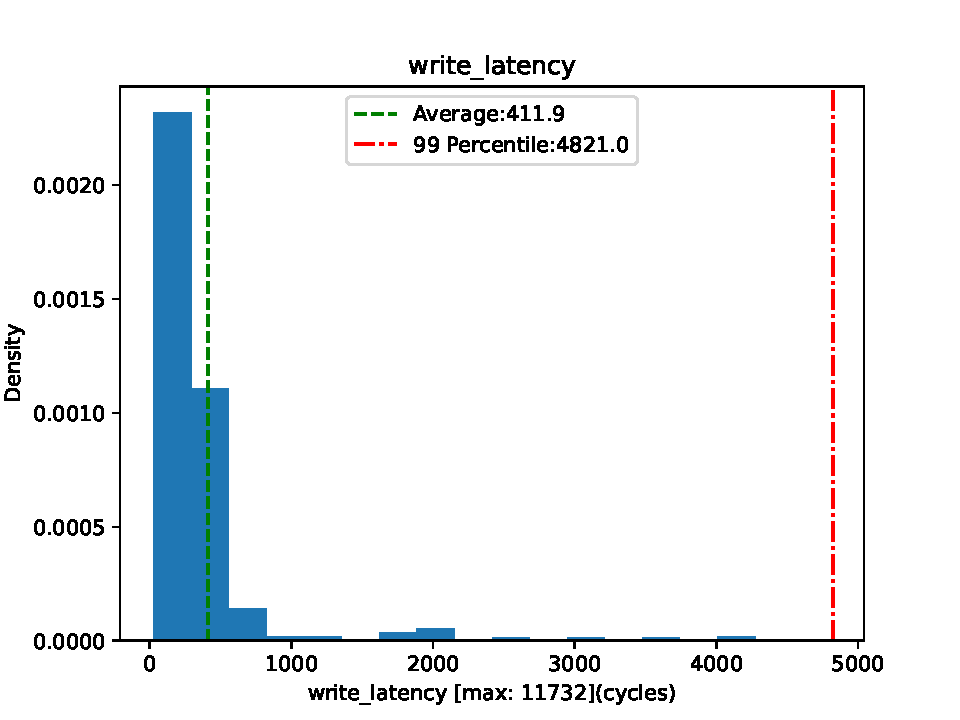
\includegraphics[height=6cm]{images/img15}
		\caption{Write latancy}
		\label{fig:Write latancy}
	\end{figure}	
\end{frame}











% --------- SECTION 4 ------- %
\section{SimpleScaler}

\begin{frame}{SimpleScaler}
	\begin{enumerate}
		\item This simulator was the doctoral thesis of Mr. Austin Todd from University of Wisconsin, which was written in C language
		
		\item This simulator is not just for memories. like Gem5, it is a system simulator.
		
		\item By default, this simulator is capable of simulating Alpha and PISA ISA. but other ISAs can also be added to it. 
		
		\item With SimpleScaler we can simulate this Micro Architecture:
		\begin{enumerate}
			\item \textbf{Sim-fast:} simulate without considering cache, pipeline and any type of micro architecture
			\item \textbf{Sim-safe:} simulate with considering access to memories
			\item \textbf{Sim-profile:} report number of simulations and dynamic instructions
			\item \textbf{Sim-cache:} simulate a system with access to cache
			\item \textbf{Sim-bpred:} report total branch prediction of program
			\item \textbf{Sim-outorder: }All the previous features are collected in this
		\end{enumerate}
	\end{enumerate}
\end{frame}



\begin{frame}{SimpleScaler (Cont.)}
	The structure of SimpleScaler is shown in bellow:
	
	\begin{figure}
		\centering
		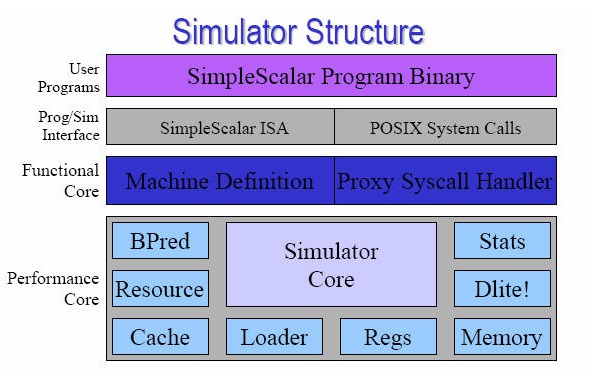
\includegraphics[height=5cm]{images/img16}
		\caption{Structure of SimpleScaler}
		\label{fig:Structure of SimpleScaler}
	\end{figure}	
\end{frame}



\begin{frame}{SimpleScaler (Cont.)}
	\textcolor{green}{Advantages:}
	\begin{enumerate}
		\item Open source
		\item System level computer with more detail
		\item Support for different architectures
	\end{enumerate}
	
	\textcolor{red}{Disadvantages:}
	\begin{enumerate}
		\item No direct access to memory
		\item Not support a new memory technologies
		\item Don't report analysis with detail like \texttt{stats} file in GEM5
	\end{enumerate}
	
\end{frame}





\begin{frame}{SimpleScaler (Cont.)}
	\textbf{How install and build SimpleScaler?}\\
	We should clone repository in first step:
	\begin{block}{Clone repository}
		\texttt{\textcolor{blue}{\$} git clone ‫‪https://github.com/stevekuznetsov/simple-scalar.git‬‬‬‬} \\
		\texttt{\textcolor{blue}{\$} ‫‪‫‪simple-scalar‬‬} \\
	\end{block}
	
	before build, we need install dependencies:
	\begin{block}{Install dependencies}
		\texttt{\textcolor{blue}{\$} sudo apt-get update‬‬} \\
		\texttt{\textcolor{blue}{\$} sudo apt-get update install build-‫‪essential‬‬‬‬} \\
		\texttt{\textcolor{blue}{\$} ‫‪sudo apt-get update install flex bison‬‬} \\
		\texttt{\textcolor{blue}{\$} ‫‪sudo apt-get update install libx11-dev‬‬} \\
	\end{block}
\end{frame}




\begin{frame}{SimpleScaler (Cont.)}
	Now we can build simulator:
	\begin{block}{Build}
		\texttt{\textcolor{blue}{\$} make config-alpha‬‬‬‬} \\
	\end{block}
	If the build is successful, your terminal output will look like this:
	
	\begin{figure}
		\centering
		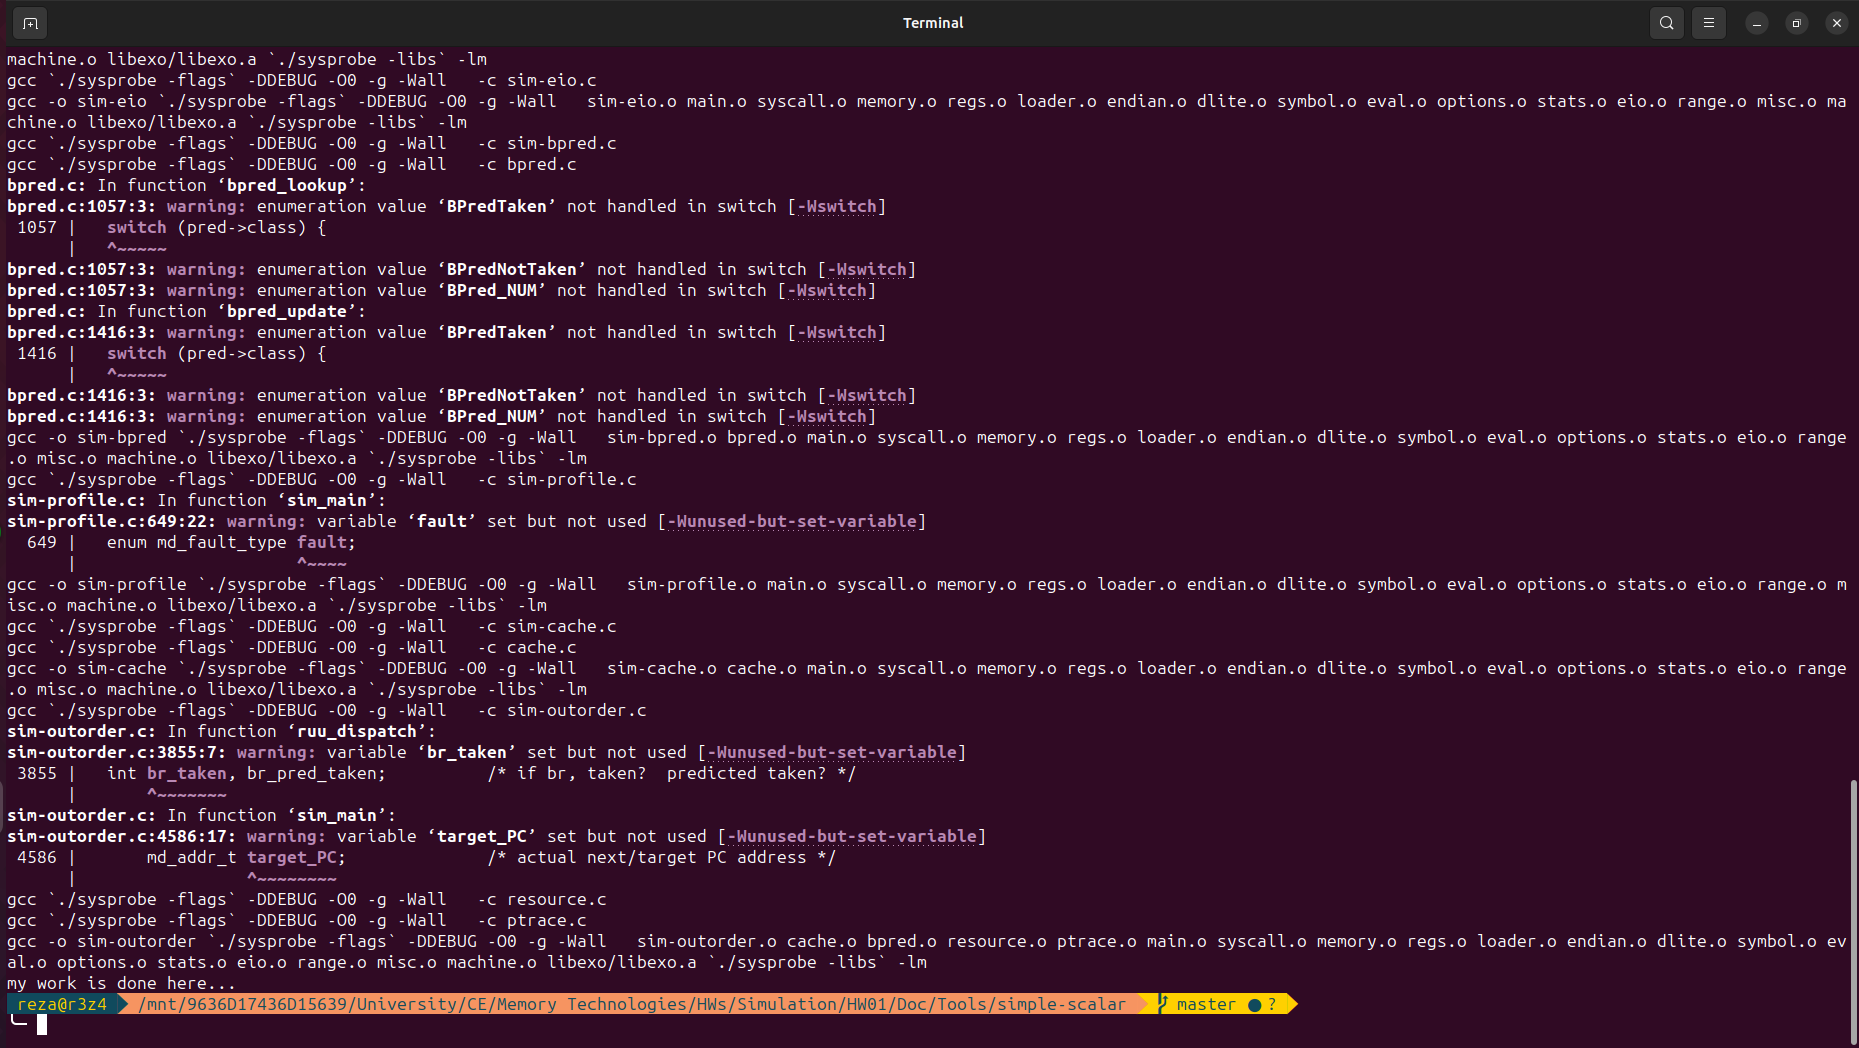
\includegraphics[height=4cm]{images/img17}
		\caption{Build successful}
		\label{fig:Build successful}
	\end{figure}
\end{frame}




\begin{frame}{SimpleScaler (Cont.)}
	\textbf{Run simulation:}\\
	The default program's \texttt{.exe} file is located in the \texttt{tests/bin/} path. also the source code of program located in \texttt{tests/src/} directory.\\
	
	in this simulation we use \texttt{test-math} program. this program calculates sine, tangent and several other mathematical operations for various inputs.
	
	Run simulation with this command:
	\begin{block}{Build}
		\texttt{\textcolor{blue}{\$} ./sim-safe tests/bin/test-math} \\
	\end{block}
\end{frame}



\begin{frame}{SimpleScaler (Cont.)}
	The output report of simulation as bellow:
	
	\begin{figure}
		\centering
		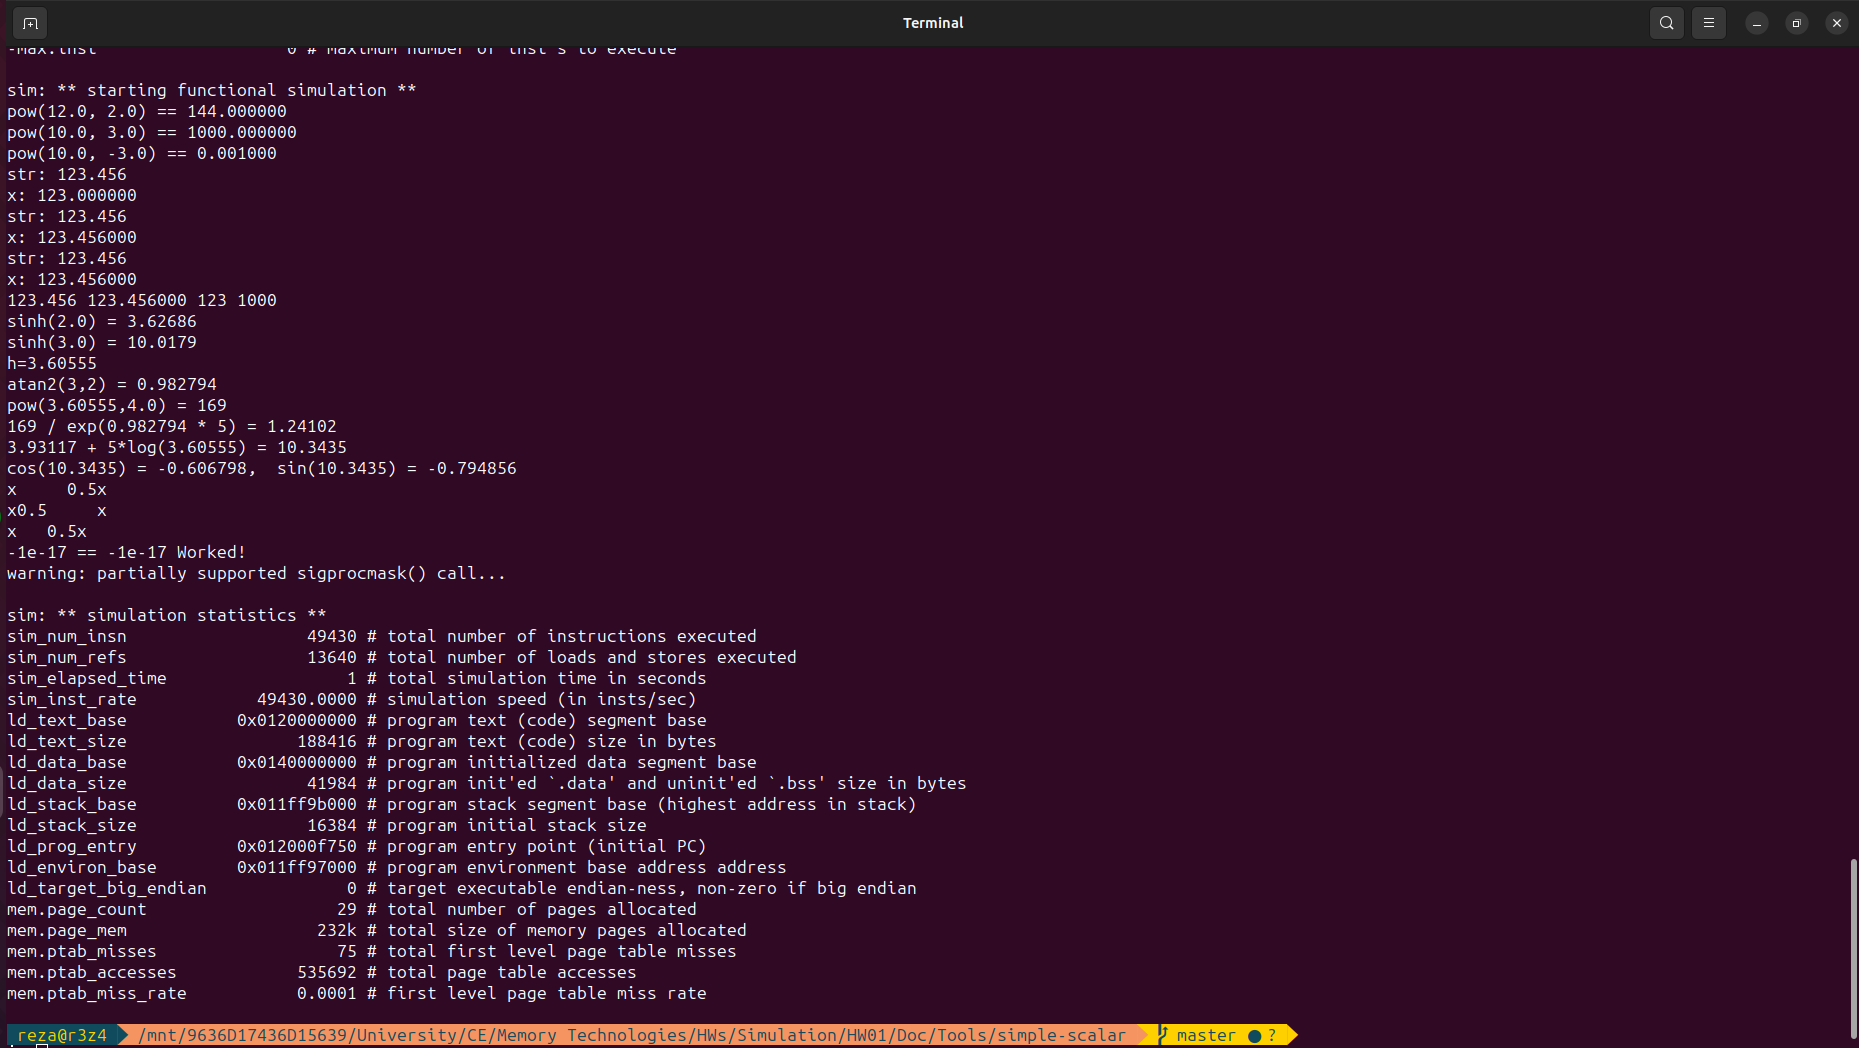
\includegraphics[height=5cm]{images/img18}
		\caption{Report of \texttt{test-math} program}
		\label{fig:Report of test-math program}
	\end{figure}
	
\end{frame}


%
%
%
%
%
%
%
%
%% --------- SECTION 4 ------- %
%\section{DRAMSIM}
%
%\begin{frame}{DRAMSIM}
%	
%	 \begin{enumerate}
%	 	\item modeling and simulation of DRAM is important because the technology tries to provide an integrated DRAM and CPU.
%	 	
%	 	\item DRAMSIM write in C++ and developed in modular based. This makes it possible to develop the Simulator and connect with other CPU Simulator like JEM5 easily.
%	 	
%	 \end{enumerate}
%
%\end{frame}
%
%
%
%
%
%
%
%
%
%
%
%
%
%
% --------- SECTION 4 ------- %
\section{References}

\begin{frame}{References}

\hyperlink{start}{\beamerreturnbutton{Back to start}}

\nocite{bibitem1}
\nocite{*}
\bibliographystyle{IEEEtran} 
\bibliography{ref}

\end{frame}






\begin{frame}[plain]
	\begin{center}
		{\Huge The End}
		
		\bigskip\bigskip % Vertical whitespace
		
		{\LARGE Questions? Comments?}\\
		You can find this slides here:\\
		\textcolor{red}{\href{https://github.com/M-Sc-AUT/M.Sc-Computer-Architecture/tree/main/Memory Technologies}{\texttt{github.com/M-Sc-AUT/M.Sc-Computer-Architecture/Memory Technologies}}}
	\end{center}
\end{frame}




\end{document}
